% Why the paper claims the drive result and not the walking result.
% Left: CPG-coupled walking, where control seeds scatter across the measured
% band. Right: the fixed-map drive readout, where no control seed reaches it.
% Values are read directly from cpg_specificity_variants.json and
% e3_body_generalization_amplitude_matched_lif.json.
\documentclass[tikz,border=3pt]{standalone}
\usepackage[T1]{fontenc}
\usepackage{xcolor}
\usetikzlibrary{calc}

\definecolor{ink}{HTML}{233747}
\definecolor{blue}{HTML}{256B91}
\definecolor{orange}{HTML}{B95020}
\definecolor{grey}{HTML}{68747D}

\begin{document}
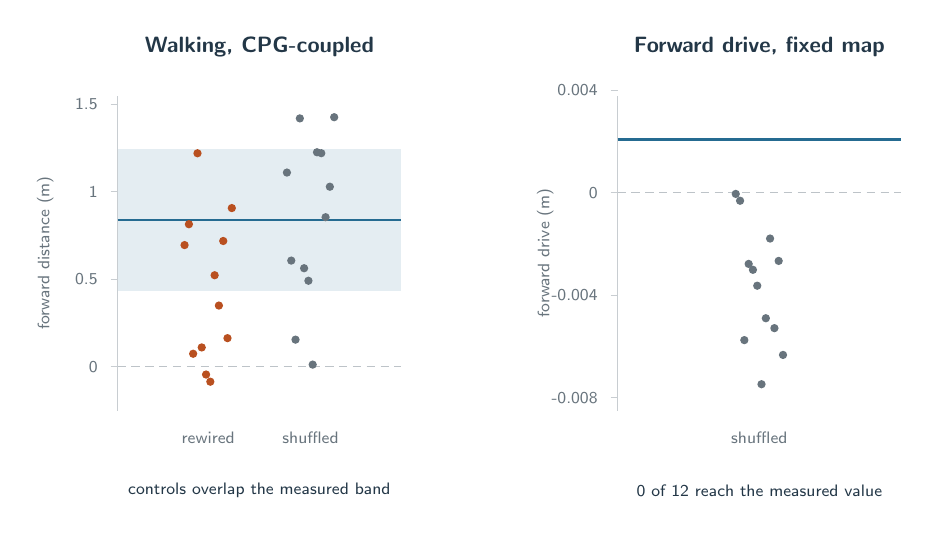
\begin{tikzpicture}[x=1cm,y=1cm,
  tick/.style={font=\sffamily\fontsize{6.4}{7.4}\selectfont,text=grey},
  note/.style={font=\sffamily\fontsize{6.4}{7.4}\selectfont,text=ink},
  ttl/.style={font=\sffamily\bfseries\fontsize{7.6}{8.8}\selectfont,text=ink}]
\begin{scope}
\draw[draw=ink!25,line width=.5pt] (0,0) -- (0,4.0);
\draw[draw=ink!25,line width=.4pt] (-.09,0.556) -- (0,0.556);
\node[tick,anchor=east] at (-.13,0.556) {0};
\draw[draw=ink!25,line width=.4pt] (-.09,1.667) -- (0,1.667);
\node[tick,anchor=east] at (-.13,1.667) {0.5};
\draw[draw=ink!25,line width=.4pt] (-.09,2.778) -- (0,2.778);
\node[tick,anchor=east] at (-.13,2.778) {1};
\draw[draw=ink!25,line width=.4pt] (-.09,3.889) -- (0,3.889);
\node[tick,anchor=east] at (-.13,3.889) {1.5};
\fill[blue,opacity=.12] (0,1.512) rectangle (3.6,3.326);
\draw[blue,line width=.9pt] (0,2.419) -- (3.6,2.419);
\draw[draw=ink!30,densely dashed,line width=.4pt] (0,0.556) -- (3.6,0.556);
\fill[orange] (0.850,2.101) circle [radius=1.5pt];
\fill[orange] (0.905,2.366) circle [radius=1.5pt];
\fill[orange] (0.959,0.721) circle [radius=1.5pt];
\fill[orange] (1.014,3.267) circle [radius=1.5pt];
\fill[orange] (1.068,0.801) circle [radius=1.5pt];
\fill[orange] (1.123,0.457) circle [radius=1.5pt];
\fill[orange] (1.177,0.366) circle [radius=1.5pt];
\fill[orange] (1.232,1.718) circle [radius=1.5pt];
\fill[orange] (1.286,1.333) circle [radius=1.5pt];
\fill[orange] (1.341,2.153) circle [radius=1.5pt];
\fill[orange] (1.395,0.919) circle [radius=1.5pt];
\fill[orange] (1.450,2.571) circle [radius=1.5pt];
\fill[grey] (2.150,3.022) circle [radius=1.5pt];
\fill[grey] (2.205,1.904) circle [radius=1.5pt];
\fill[grey] (2.259,0.900) circle [radius=1.5pt];
\fill[grey] (2.314,3.710) circle [radius=1.5pt];
\fill[grey] (2.368,1.807) circle [radius=1.5pt];
\fill[grey] (2.423,1.648) circle [radius=1.5pt];
\fill[grey] (2.477,0.583) circle [radius=1.5pt];
\fill[grey] (2.532,3.280) circle [radius=1.5pt];
\fill[grey] (2.586,3.268) circle [radius=1.5pt];
\fill[grey] (2.641,2.455) circle [radius=1.5pt];
\fill[grey] (2.695,2.842) circle [radius=1.5pt];
\fill[grey] (2.750,3.725) circle [radius=1.5pt];
\node[tick,align=center] at (1.15,-.34) {rewired};
\node[tick,align=center] at (2.45,-.34) {shuffled};
\node[ttl] at (1.80,4.62) {Walking, CPG-coupled};
\node[tick,rotate=90] at (-.92,2.00) {forward distance (m)};
\node[note,align=center] at (1.8,-1.02) {controls overlap the measured band};
\end{scope}
\begin{scope}[shift={(6.35,0)}]
\draw[draw=ink!25,line width=.5pt] (0,0) -- (0,4.0);
\draw[draw=ink!25,line width=.4pt] (-.09,0.163) -- (0,0.163);
\node[tick,anchor=east] at (-.13,0.163) {-0.008};
\draw[draw=ink!25,line width=.4pt] (-.09,1.463) -- (0,1.463);
\node[tick,anchor=east] at (-.13,1.463) {-0.004};
\draw[draw=ink!25,line width=.4pt] (-.09,2.764) -- (0,2.764);
\node[tick,anchor=east] at (-.13,2.764) {0};
\draw[draw=ink!25,line width=.4pt] (-.09,4.065) -- (0,4.065);
\node[tick,anchor=east] at (-.13,4.065) {0.004};
\draw[blue,line width=.9pt] (0,3.440) -- (3.6,3.440);
\draw[draw=ink!30,densely dashed,line width=.4pt] (0,2.764) -- (3.6,2.764);
\fill[grey] (1.500,2.751) circle [radius=1.5pt];
\fill[grey] (1.555,2.664) circle [radius=1.5pt];
\fill[grey] (1.609,0.894) circle [radius=1.5pt];
\fill[grey] (1.664,1.862) circle [radius=1.5pt];
\fill[grey] (1.718,1.787) circle [radius=1.5pt];
\fill[grey] (1.773,1.585) circle [radius=1.5pt];
\fill[grey] (1.827,0.334) circle [radius=1.5pt];
\fill[grey] (1.882,1.172) circle [radius=1.5pt];
\fill[grey] (1.936,2.184) circle [radius=1.5pt];
\fill[grey] (1.991,1.046) circle [radius=1.5pt];
\fill[grey] (2.045,1.900) circle [radius=1.5pt];
\fill[grey] (2.100,0.706) circle [radius=1.5pt];
\node[tick,align=center] at (1.8,-.34) {shuffled};
\node[ttl] at (1.80,4.62) {Forward drive, fixed map};
\node[tick,rotate=90] at (-.92,2.00) {forward drive (m)};
\node[note,align=center] at (1.8,-1.02) {0 of 12 reach the measured value};
\end{scope}
\end{tikzpicture}
\end{document}
